% T. Padmanabhan Solutions Manual

\documentclass{report}
\usepackage[paperwidth=16cm, paperheight=21cm, top = 20mm, bottom = 18mm, left=10mm, right = 10mm]{geometry}
\usepackage{fancyhdr}
\pagestyle{fancy}

\usepackage{graphicx}
\usepackage{amsmath, amsfonts, amssymb, amsthm}
\usepackage{tensor}
\usepackage{physics}
\usepackage{cancel}
\usepackage{hyphenat}
\usepackage{hyperref}
\usepackage{pgfplots}
\hypersetup{colorlinks, linkcolor = [RGB]{66, 128, 128}, urlcolor = red, linktocpage = true}
\usepackage{enumitem}

% \usepackage{charter}

\DeclareMathOperator{\arctanh}{arctanh}

\newlist{subquests}{enumerate}{2}
\setlist[subquests, 1]{leftmargin=*, label = \textbf{\arabic*.}}
\setlist[subquests, 2]{leftmargin=*, label = (\alph*)}

\renewcommand{\familydefault}{\sfdefault}

\begin{document}

\title{Solutions to \\ Gravitation: Foundations and Frontiers \\ by T. Padmanabhan}

\author{Arjit Seth}
\date{}

\maketitle

\chapter{Special relativity}


\begin{subquests}
	\item \emph{Light clocks.}
	Perpendicular:
	\begin{align*}
		ct' & = \sqrt{c^2 - v^2}t \\
		t & = \frac{t'}{\sqrt{1 - v^2/c^2}} = \gamma t'
	\end{align*}
	Parallel: Using proper time -
	\begin{align*}
		\dd{t} & = \gamma\dd{\tau} \\ 
		\frac{L'}{c+v} + \frac{L'}{c-v}  & = \gamma\frac{2L}{c} \\
		L'\frac{2c}{c^2 - v^2} & = \gamma\frac{2L}{c} \\
		L' & = L \frac{1-v^2/c^2}{\sqrt{1-v^2/c^2}} = \frac{L}{\gamma} \\
	\end{align*}

	\item \emph{Superluminal motion.}
	\begin{align*}
		\Delta t' & = t_2' - t_1' \\
		t_1' - t_1 & \approx \frac{v}{c}\Delta t \cos\theta \\
		t_2' - t_1 & = L/c \\
		\Delta t' & = \Delta t\pqty{1-(v/c)\cos\theta} \\
		v_{app} & = v\Delta t \sin\theta = \frac{v\sin\theta}{1-(v/c)\cos\theta}
	\end{align*}
	Rewriting this expression and plotting it for $v = 0.99 c$:
	\begin{align*}
		v_{app} = \frac{v\sqrt{1 - \cos^2 \theta}}{1-v\cos\theta}, \quad c = 1
	\end{align*}
	% \begin{center}
	% 	\begin{tikzpicture}[domain = 0:2*pi]
	% 		\begin{axis}
	% 			\addplot[color=blue]{sqrt(0.99*1-(cos (deg(x)))^2)/(1-0.99*(cos (deg(x))))};
	% 		\end{axis}
	% 	\end{tikzpicture}
	% \end{center}

	\item \emph{The strange world of four-vectors.}
	\begin{subquests}
		\item This is evident from taking the inner product, since the magnitudes add up.
		\begin{align*}
			\pqty{a^i + b^i}\pqty{a_i + b_i} = a^i a_i + b^i b_i + 2\pqty{a^i b_i}
		\end{align*}

		\item Let $k^i$ be a non-zero null vector. If non-zero $a^i$ is a vector orthogonal to $k^i$, then $a_i k^i = 0$.  
	\end{subquests}

	\item \emph{Focused to the front.}
	\begin{subquests}
		\item
		Using a Lorentz transformation on the `time' and `space' components of the four-vector $k^a = (\omega,\omega{\bf n}/c)$:
		\begin{align*}
			\omega_R & = \gamma\bqty{\omega_L - \frac{\omega_Lv\cos\theta_L}{c}} = \gamma\omega_L\pqty{1-(v/c)\cos\theta_L} \\
			\omega_R \cos\theta_R & = \gamma\bqty{\omega_L \cos\theta_L - \frac{\omega_Lv}{c}} = \gamma\omega_L\bqty{\cos\theta_L - (v/c)} \\
			\frac{\omega_R \cos\theta_R}{\omega_R} & = \frac{\gamma\omega_L\bqty{\cos\theta_L - (v/c)}}{\gamma\omega_L\bqty{1-(v/c)\cos\theta_L}} \\
			\mu_R & = \frac{\mu_L- (v/c)}{1-(v\mu_L/c)}
		\end{align*}

		\item 
		\begin{center}
			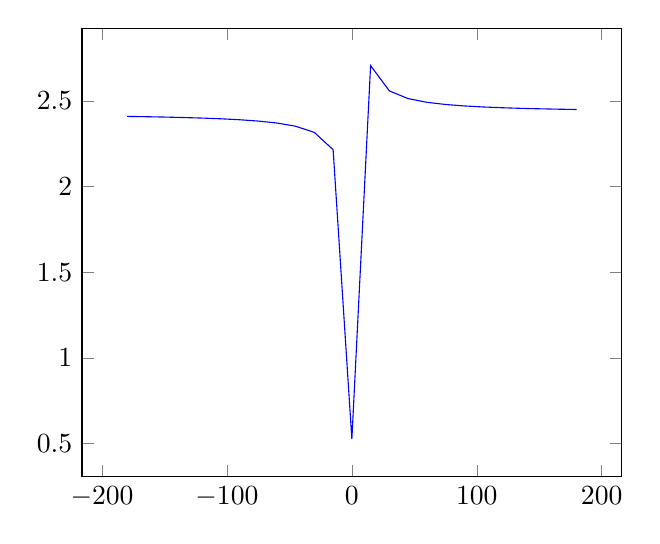
\begin{tikzpicture}[domain = -180:180]
				\begin{axis}
					\addplot[color=blue]{(cos(deg(45)) - x/(1-x*(cos(deg(45))))};
				\end{axis}
			\end{tikzpicture}
		\end{center}

		\item The solid angle is found by taking the differential of $\mu_R$:
		\begin{align*}
			\dd{\Omega} & = \int\sin\theta\dd{\theta}\dd{\phi} = -\int\dd(\cos\theta)\dd{\phi} \\
			\dd(\cos\theta_R) & = \bqty{\frac{(v/c)\bqty{\cos\theta_L - (v/c)}}{\bqty{1-(v/c)\cos\theta_L}^2} + \frac{1}{\bqty{1-(v/c)\cos\theta_L}}}\dd(\cos\theta_L) \\
			\dd{\Omega'} & = \frac{1}{\gamma^2}\frac{\dd{\Omega}}{\bqty{1-(v/c)\cos\theta}^2}
		\end{align*}
		The energy is:
		\begin{align*}
			\dd{\mathcal E'} = \hbar \omega = \gamma \dd{\mathcal E}\bqty{1-(v/c)\cos \theta} 
		\end{align*}
		The time is:
		\begin{align*}
			\dd{t'} = \gamma \dd{t}
		\end{align*}
		Therefore, the energy emitted per unit time into a given solid angle in the rest frame is $(c=1)$:
		\begin{align*}
			\pqty{\frac{\dd{\mathcal E'}}{\dd{t'}{\dd\Omega'}}}_{\mathrm{rest}} & = \gamma^2\pqty{1-v\cos\theta}^3\pqty{\frac{\dd{\mathcal E}}{\dd{t}\dd{\Omega}}}_{\mathrm{lab}} \\
			\pqty{\frac{\dd{\mathcal E}}{\dd{t}\dd{\Omega}}}_{\mathrm{lab}} & = \frac{\pqty{1-v^2}^2}{\pqty{1-v\cos\theta}^3}\pqty{\frac{\dd{\mathcal E'}}{\dd{t'}{\dd\Omega'}}}_{\mathrm{rest}}
		\end{align*}
		If the emission is isotropic, $\dd{\Omega} = \dd{\Omega'} = 4\pi$:
		\begin{align*}
			\pqty{\dv{\mathcal E}{t}}_{\mathrm{lab}}  = \dd{\Omega}\pqty{\frac{\dd{\mathcal E'}}{\dd{t'}{\dd\Omega'}}}_{\mathrm{rest}} = \pqty{\dv{\mathcal E'}{t'}}_{\mathrm{rest}}
		\end{align*}
	\end{subquests}

	\item \emph{Transformation of antisymmetric tensors.}
	\begin{align*}
		A^{i'k'} = L^{k'}_k L^{i'}_i A^{ik} = \pdv{x^{k'}}{x^k}\pdv{x^{i'}}{x^i}A^{ik}
	\end{align*}
	If $A^{ik} = -A^{ki}$ then:
	\begin{align*}
		A^{k'i'} = - A^{i'k'} ?
	\end{align*}

	\item \emph{Practice with completely antisymmetric tensors.}
	\begin{subquests}
		\item 

		\item Multiplying each index by the metric tensor:
		\begin{gather*}
			\epsilon^{abcd} = g^{ai}g^{bj}g^{ck}g^{dl}\epsilon_{ijkl} = 
		\end{gather*}

		\item

		\item
	\end{subquests}
	\item \emph{A null curve in flat spacetime.}
	\begin{align*}
		\eta_{ij}x^{i}x^{j} = -t^2 + x^2 + y^2 + z^2 = 0 
	\end{align*}

	\item \emph{Shadows are Lorentz invariant.}

	\item \emph{Hamiltonian form of action - Newtonian mechanics.}
	\begin{align*}
		\mathcal A & = \int_{t_2}^{t_1}\dd{t}\,\bqty{p\dot q - H(p,q)} \\
		\delta\mathcal A & = \int_{t_2}^{t_1} \dd{t}\, \bqty{\dot q\,\delta p + p\,\delta\dot q  - \pdv{H}{p}\delta p - \pdv{H}{q}\delta q} = 0
	\end{align*}
	Using $\delta\dot q = \dot\dd(\delta q)$ and integrating by parts:
	\begin{gather*}
		\int_{t_2}^{t_1} \dd{t}\, p\,\delta \dot q = \cancel{\left|p\,\delta q\right|_{t_1}^{t_2}} - \int_{t_2}^{t_1} \dd{t}\,\dot p\, \delta q  \\
		\therefore \int_{t_2}^{t_1} \dd{t}\, \bqty{\pqty{\dot q -\pdv{H}{p}}\,\delta p - \pqty{\dot p + \pdv{H}{q}}\delta q} = 0
	\end{gather*}
	Since $\delta q = 0 $ at the endpoints, the second term is zero; therefore, the first term in parentheses should be zero, leading to the equations of motion:
	\begin{align*}
		\dot q = \pdv{H}{p},\;\;\;\dot p = -\pdv{H}{q} 	
	\end{align*} 
	
	\item \emph{Hamiltonian form of action - special relativity.}
	\begin{align*}
		\mathcal A & = \int_{\lambda_1}^{\lambda_2} \dd{\lambda}\, \bqty{p_a \dot x^a - \frac{1}{2}C\pqty{\frac{H}{mc^2} + mc^2}}, \quad H = \eta_{ab} p^a p^b \\
		\delta\mathcal A & = \int_{\lambda_1}^{\lambda_2}\delta p_a \dot x^a + p_a \delta\dot x^a -\frac{1}{2}\bqty{\delta C\pqty{\frac{H}{m} + m} + C\pqty{\frac{2p^a\delta p_a}{mc^2}}} \dd{\lambda} = 0 \\
		& = \int_{\lambda_1}^{\lambda_2} \bqty{\dot x^a - \frac{C}{m}p^a}\delta p_a - \dot p_a\delta x^a - \frac{1}{2}\bqty{\frac{H + m^2}{m}}\delta C \dd{\lambda} = 0, \quad c = 1
	\end{align*}

	\item \emph{Hitting a mirror.}

	\item \emph{Photon-electron scattering.}

	\item \emph{More practice with collisions.}

	\item \emph{Relativistic rocket.}

	\item \emph{Practice with equilibrium distribution functions.}

	\item \emph{Projection effects.}

	\item \emph{Relativistic virial theorem.}
	The conservation law implies the following:
	\begin{align*}
		\partial_0 T^{00}x^{\alpha}x^{\beta} & = -\partial_{\mu}T^{0\mu}x^{\alpha}x^{\beta} \\
		& = -\partial_{\mu}\bqty{T^{0\mu}x^{\alpha}x^{\beta}} + T^{0\mu}\partial_{\mu}\bqty{x^{\alpha}x^{\beta}} \\
		& = -\partial_{\mu}\bqty{T^{0\mu}x^{\alpha}x^{\beta}} + T^{0\mu}\bqty{\partial_{\mu}x^{\alpha}x^{\beta} + x^{\alpha}\partial_{\mu}x^{\beta}} \\
		& =  -\partial_{\mu}\bqty{T^{0\mu}x^{\alpha}x^{\beta}} + T^{0\alpha}x^{\beta} + T^{0\beta}x^{\alpha}
	\end{align*}
	Taking the time derivative and using the fact that partial derivatives commute:
	\begin{align*}
		\partial_0\pqty{\partial_0 T^{00}}x^{\alpha}x^{\beta} & = -\partial_{\mu}\bqty{\partial_0 T^{0\mu}}x^{\alpha}x^{\beta} \\
		\partial^2_0 T^{00}x^{\alpha}x^{\beta} & = -\partial_{\mu}\bqty{\partial_0 T^{0\mu}x^{\alpha}x^{\beta}} + \partial_0 T^{0\alpha}x^{\beta} + \partial_0 T^{0\beta}x^{\alpha} \\
		& = -\partial_{\mu}\bqty{\partial_0 T^{0\mu}x^{\alpha}x^{\beta}} - \partial_{\nu}T^{\nu\alpha}x^{\beta} - \partial_{\nu}T^{\nu\beta}x^{\alpha}, \quad \pqty{\partial_i T^{i\alpha} = 0} \\
		& = -\partial_{\mu}\bqty{\partial_0 T^{0\mu}x^{\alpha}x^{\beta} + T^{\mu\alpha}x^{\beta} + T^{\mu\beta}x^{\alpha}} + 2 T^{\alpha\beta}, \quad \pqty{T^{\mu\alpha}\partial_{\mu}x^{\beta} = T^{\alpha\beta}}
	\end{align*}
	Integrating both sides of the equation and using the divergence theorem for the condition that $T^{ij} = 0$ outside a compact region in space:
	\begin{gather*}
		\int \dd^3{x}\;\partial^2_0 T^{00} x^{\alpha}x^{\beta} = \int \dd^3{x} \bqty{-\partial_{\mu}\pqty{\partial_0 T^{0\mu}x^{\alpha}x^{\beta} + T^{\mu\alpha}x^{\beta} + T^{\mu\beta}x^{\alpha}} + 2 T^{\alpha\beta}} \\
		\therefore \dv[2]{t}\int \dd^3{x}\;T^{00} x^{\alpha} x^{\beta} = 2 \int \dd^3{x}\; T^{\alpha\beta}
	\end{gather*}

	\item \emph{Explicit computation of spin precession.}
	The four-velocity and four-acceleration are:
	\begin{align*}
		u^i = \pqty{\gamma, \gamma \vb v} = \pqty{\gamma, -\gamma r\omega\sin\omega t, \gamma r\omega\cos\omega t, 0} \\
		a^i = \gamma\pqty{\dot{\gamma}, \dot{\gamma}\vb v + \dot{\vb v}\gamma} = -\gamma^2 \omega^2\pqty{0,x,y,0}
	\end{align*}
	Using the equation of motion for a moving particle with spin and separating the space and time components:
	\begin{align*}
		\dv{S^j}{\tau} & = u^j \pqty{S^k a_k} \\
		S^k a_k & = -\gamma^2 \omega^2 \pqty{xS^x + yS^y} \\
		\dv{t}\bqty{\pqty{yS^x - xS^y}} & = -\omega\pqty{xS^x + yS^y}
	\end{align*}

	\item \emph{Little group of the Lorentz group.}
\end{subquests}


\chapter{Scalar and electromagnetic fields in special relativity}

\begin{subquests}
	\item \emph{Measuring the $F^{ab}$.}

	\item \emph{Schr\"odinger equation and gauge transformation.}
	The transformed Schr\"odinger equation is:
	\begin{align*}
		i\hbar\partial_t \psi = \bqty{\frac{1}{2m}\bqty{\mathbf{P} - \frac{q}{c}\pqty{\mathbf A + \nabla f}}^2 + q\pqty{\phi + \partial_t f}}\psi
	\end{align*}

	\item \emph{Four-vectors leading to electric and magnetic fields.}
	\begin{subquests}
		\item Taking dot products:
		\begin{gather*}
			E^i u_i = F^{ij}u_j u_i = 0 \\
			B^a u_a = \frac{1}{2}\epsilon^{abcd}F_{cd}u_a u_b = \frac{1}{2}(*F)^{ab}u_a u_b = 0
		\end{gather*}
		since $u_i u_j$ is symmetric and $F^{ij}$ and its dual are antisymmetric.

		\item
	\end{subquests}

	\item \emph{Hamiltonian form of action - charged particle.}
	\begin{align*}
		\mathcal A & = \int_{\lambda_1}^{\lambda_2} \bqty{P_a \dot x^a - \frac{1}{2}C\pqty{\frac{H}{mc^2} + mc^2}}, \quad H = \eta_{ij}\pqty{P^i - qA^i}\pqty{P^j - qA^j} \\
		\delta\mathcal A & = \int_{\lambda_1}^{\lambda_2}\delta P_a \dot x^a + P_a \delta\dot x^a -\frac{1}{2}\bqty{\delta C\pqty{\frac{H}{m} + m} + C\pqty{\frac{\pqty{P^i - qA^i}\pqty{\delta P_i -q \delta A_j}}{mc^2}}} \dd{\lambda} = 0 
	\end{align*}

	\item \emph{Three-dimensional form of the Lorentz force.}
	Using the electromagnetic tensor equation of motion $u^i = (\gamma c, \gamma \vb v)$:
	\begin{align*}
		m\dv{u^i}{\tau} = q F^{ik}u_k & \implies mc\gamma\dv{u^0}{t} = q F^{0\alpha}u_{\alpha}, \quad \dv{u^0}{\tau} = \gamma \dv{u^0}{t} \\
		mc\gamma\dv{\gamma}{t} = q\gamma\bqty{(\mathbf E/c) \cdot \mathbf v} & \implies \frac{1}{\gamma^3}\pqty{m\mathbf v\cdot\dv{\mathbf v}{t}} = q\pqty{\mathbf E \cdot \mathbf v}, \quad \dv{\gamma}{t} = \frac{1}{\gamma^3}\pqty{\frac{\vb v}{c^2}\cdot \dv{\vb v}{t}}  \\
		m\dv{u^{\alpha}}{t} & = q F^{\alpha\beta}u_{\beta} = q\pqty{\mathbf E + \mathbf v \times \mathbf B} \\
		\bqty{\frac{1}{\gamma^3}\pqty{\frac{m\mathbf v}{c^2}\cdot \dv{\mathbf v}{t}}\vb v + m\gamma \dv{\mathbf v}{t}} & = q\pqty{\mathbf E + \mathbf v \times \mathbf B} \\
		\implies \dv{\mathbf v}{t} & = \frac{q}{m\gamma}\bqty{\mathbf E + \mathbf v \times \mathbf B - \frac{1}{c^2}\pqty{\mathbf E \cdot \mathbf v}\mathbf v}
	\end{align*}

	\item \emph{Pure gauge impostors.}
	This can be transformed into polar coordinates ($x = \cos\theta, y = \sin\theta $) and evaluated ($A_r = 0$, obviously):
	\begin{align*}
		A_{\theta} = \pdv{f}{\theta} = \pdv{f}{x}\pdv{x}{\theta} + \pdv{f}{y}\pdv{y}{\theta} = 1,\\
		\oint\limits_{C = x^2 + y^2} \mathbf A \cdot \dd{\mathbf s} = \int_0^{2\pi}\dd{\theta} = 2\pi 
	\end{align*}
	The reason why $\mathbf A$ is not a pure gauge mode is because $f$ is singular at the origin, making it non-differentiable at that point. It is also a non-removable singularity, so no analytic continuation can be performed.

	\item \emph{Pure electric or magnetic fields.}

	\item \emph{Elegant solution to non-relativistic Coulomb motion.}
	\begin{subquests}
		\item
		Since the angular momentum is conserved, $\dd{\mathbf J}/\dd{t} = 0$:
		\begin{align*}
			\dv{t}\pqty{\mathbf p \times \mathbf J} & = \dv{\mathbf p}{t}\times \mathbf J + \cancel{\mathbf p \times \dv{\mathbf J}{t}} \\
			f(r)\hat{\mathbf r} \times \mathbf r \times m\mathbf v & = mf(r)\bqty{\mathbf r\pqty{\cancel{\hat{\mathbf r}\cdot \mathbf v}} - \mathbf v\pqty{\hat{\mathbf r}\cdot \mathbf r}} \\
			& = -mf(r)r\dv{\mathbf r}{t} = -mf(r)r^2 \dv{\hat{\mathbf r}}{t}  
		\end{align*}
		Therefore, if $f(r)r^2 = -\abs{\alpha}$, then:
		\begin{align*}
			\int \frac{1}{m\abs{\alpha}}\dv{t}\pqty{\mathbf p \times \mathbf J} \dd{t} & = \int \dv{\hat{\mathbf r}}{t} \dd{t} \\
			\implies \frac{\mathbf p \times \mathbf J}{m\abs{\alpha}} - \hat{\mathbf r} & = \mathbf e
		\end{align*}
		where $\mathbf e$ is a conserved vector, arising as a constant of the integration. \\
		
		\item Note that $\mathbf p$ and $\mathbf J$ are perpendicular:
		\begin{align*}
			\mathbf e \cdot \mathbf e & = \bqty{\frac{\mathbf p \times \mathbf J}{m\abs{\alpha}} - \hat{\mathbf r}}\cdot \bqty{\frac{\mathbf p \times \mathbf J}{m\abs{\alpha}} - \hat{\mathbf r}} \\
			\implies \abs{\mathbf e}^2 & = \frac{\abs{\mathbf p \times \mathbf J}^2}{m^2\abs{\alpha}^2} - 2\pqty{\frac{\hat{\mathbf r} \cdot \mathbf p \times \mathbf J}{m\abs{\alpha}}} + 1 \\
			& = \frac{p^2 J^2}{m^2\abs{\alpha}^2}- 2\pqty{\frac{J^2}{m\abs{\alpha}r}} + 1, \quad J^2 = \pqty{\mathbf r \times \mathbf p} \cdot \mathbf J\\
			& = 1 + \frac{2EJ^2}{m\abs{\alpha}^2}, \;\; E = \frac{p^2}{2m} - \frac{\abs{\alpha}}{r}
		\end{align*}
		
		\item
		\begin{align*}
			\mathbf e \cdot \mathbf r & = \frac{\mathbf r \cdot \mathbf p \times \mathbf J}{m\abs{\alpha}} - \mathbf r \cdot \hat{\mathbf r} \\
			er\cos\theta & = \frac{J^2}{m\abs{\alpha}} - r \\
			\implies r(\theta) & = \frac{J^2/m\abs{\alpha}}{1+ e\cos\theta}
		\end{align*}

		\item
		\begin{align*}
			E = \frac{p^2}{2m} - \frac{\abs{\alpha}}{r} - \frac{\abs{\beta}}{r^2}
		\end{align*}
	\end{subquests}

	\item \emph{More on uniformly accelerated motion.}

\end{subquests}
	
\chapter{Gravity and spacetime geometry: the inescapable connection}


\chapter{Metric tensor, geodesics and covariant derivative}

\begin{subquests}
	\item \emph{Practice with metrics.}
	\begin{subquests}
		\item $x = 2\tan(\theta/2)\cos\phi, y = 2\tan(\theta/2)\sin\phi$. Since the coordinates are spherical:
		\begin{align*}
			g_{ab} & = \eta_{ij}\pdv{X^i}{x^a}\pdv{X^j}{x^b}, \quad X^i = \theta,\,\phi,\; x^a = x,\,y, \;\eta_{ij} = \mqty[1 & 0 \\ 0 & \sin^2\theta]  \\
			\pdv{\theta}{x^a} & = \pdv{x^a}\bqty{2\tan^{-1}\pqty{\frac{\sqrt{x^2 + y^2}}{2}}}, \quad \pdv{\phi}{x^a} = \pdv{x^a}\bqty{\tan^{-1}\pqty{y/x}} \\
			\pdv{\theta}{x^a} & = \frac{4x^a}{\sqrt{x^2 + y^2}\pqty{x^2 + y^2 + 4}} = \cos^2\pqty{\theta/2}\cos\phi,\;\cos^2\pqty{\theta/2}\sin\phi \\
			\quad \pdv{\phi}{x} & = -\frac{y}{x^2 + y^2} = -\frac{\sin\phi}{2\tan\pqty{\theta/2}}, \quad \pdv{\phi}{y}  = \frac{x}{x^2 + y^2} = \frac{\cos\phi}{2\tan\pqty{\theta/2}} \\
			g_{xx} & = \pqty{\pdv{\theta}{x}}^2 + \sin^2\theta\pqty{\pdv{\phi}{x}}^2 \\
			& = \bqty{\cos^2\pqty{\theta/2}\cos^2\phi + \frac{\sin^2\theta\sin^2\phi}{4\sin^2\pqty{\theta/2}}}\cos^2\pqty{\theta/2} = \cos^4(\theta/2) \\
			g_{yy} & = \pqty{\pdv{\theta}{y}}^2 + \sin^2\theta\pqty{\pdv{\phi}{y}}^2 \\
			& = \bqty{\cos^2(\theta/2)\sin^2\phi + \frac{\sin^2\theta\cos^2\phi}{4\sin^2{\theta/2}}}\cos^2(\theta/2) = \cos^4(\theta/2) \\
			\therefore \dd{s}^2 & = \cos^4\pqty{\frac{\theta}{2}}\bqty{\dd x^2 + \dd y^2}
		\end{align*}
	\end{subquests}
\end{subquests}

\end{document}